\subsection{Das konzeptionelle Modell der Webseite}
    Abbildung \ref{image:findingNewsModelOverview} zeigt einen
    Ausschnitt der zu klassifizierenden Webseite,
    anhand dessen das konzeptionelle Modell der Seite erläutert wird.
    Eine Darstellung des Modells ist außerdem in Abbildung
    \ref{image:findingNewsModelUml} zu sehen.

    \begin{figure}[htb]
        \centering
        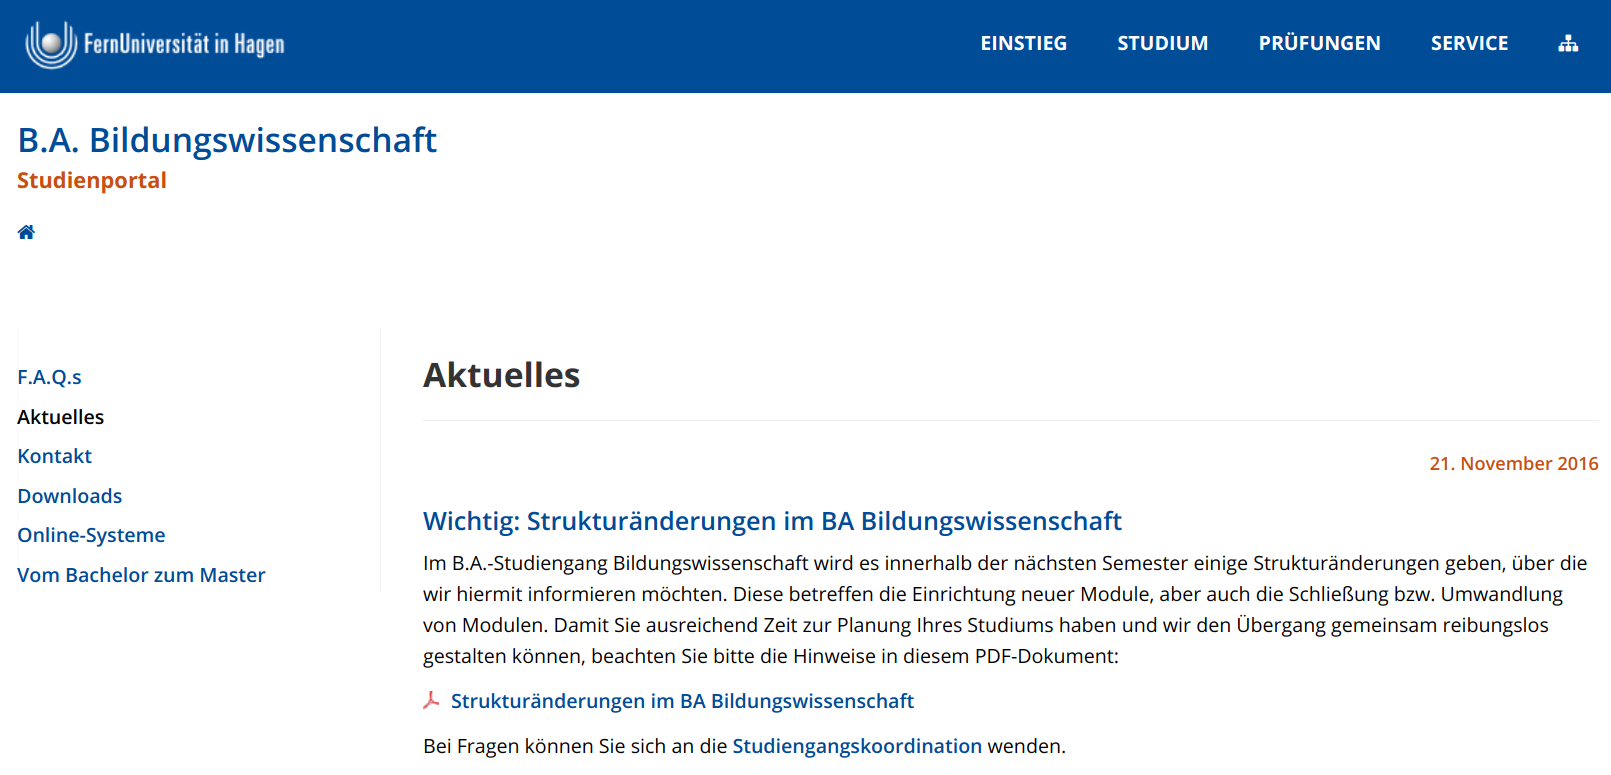
\includegraphics[width=\textwidth]{../resources/findings/case-study-2/news-overview.png}
        \caption{Aktuelle Meldungen im Portal \acrshort{babw}}
        \label{image:findingNewsModelOverview}
    \end{figure}

    Es ist leicht zu erkennen, dass es auf dieser Webseite einige Überschneidungen
    mit der des vorherigen Beispiels gibt.
    Das betrifft den Kopfbereich, den Namen des Portals,
    die seitlichen Navigationspunkte und die Überschrift der Seite.
    Im Vergleich zum ersten Beispiel gibt es hier nur wenige inhaltliche,
    aber keine konzeptionellen Unterschiede,
    weshalb auf diese Bereiche nicht weiter eingegangen wird und Abbildung
    \ref{image:findingNewsModelUml} sie nicht modelliert.
    Unterschiede werden erst im mittleren Bereich ersichtlich,
    wo die Auflistung der einzelnen Nachrichten erfolgt.
    Jede Nachricht besitzt ein Datum, eine Überschrift und beliebig viele Absätze,
    die ihrerseits Text, Links usw. enthalten.
    Die Überschrift ist gleichzeitig auch ein Link auf die Einzelseite der Meldung.
    Die Meldungen des Portals werden nicht alle auf einer Nachrichtenseite dargestellt,
    sondern auf mehrere verteilt.
    Zwei Links, die in Abbildung \ref{image:findingNewsModelOverview} nicht zu sehen sind,
    führen einen Besucher der Webseite zur nächsten bzw. vorherigen Übersichtsseite.
    Dabei handelt es sich um eigenständige Seiten mit individuellen \glspl{url},
    die aber alle dem beschriebenen Modell folgen.

    \begin{figure}[htb]
        \centering
        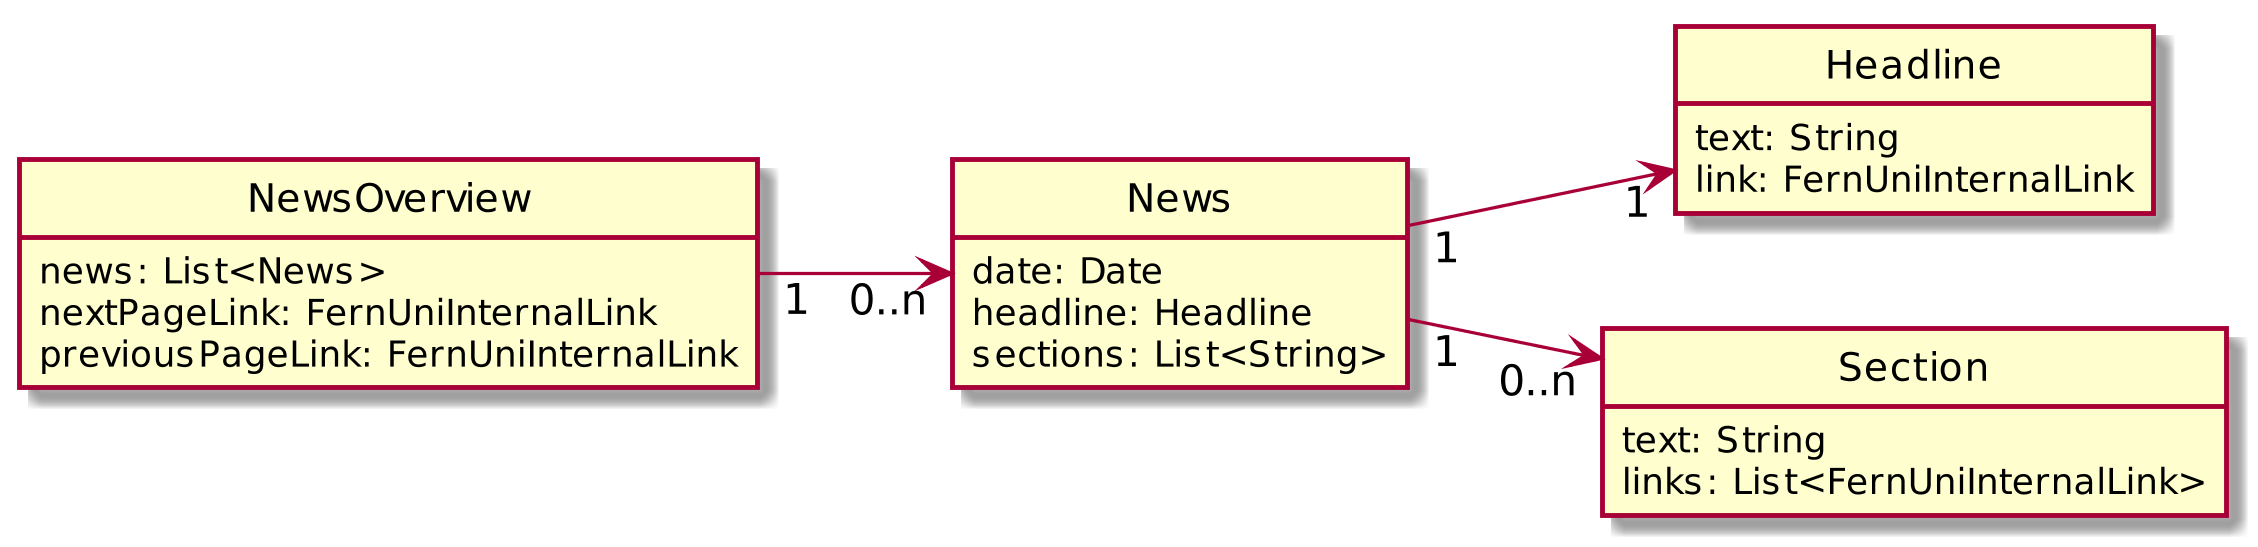
\includegraphics[scale=\imageScalingFactor]{../resources/findings/case-study-2/model.png}
        \caption{Konzeptionelles Modell der Seite über aktuelle Meldungen}
        \label{image:findingNewsModelUml}
    \end{figure}